\documentclass[pdftex,12pt,xcolor=svgnames]{beamer}

\mode<presentation>
{
  \usetheme{boxes}
  \usecolortheme[named=MidnightBlue]{structure}
  %\setbeamercolor{normal text}{bg=NavajoWhite!20}
  \usefonttheme{serif}
  \setbeamertemplate{navigation symbols}{}
  % Show frame number and author name in footline
  \setbeamertemplate{footline}[frame number]
  \addtobeamertemplate{footline}{\quad\textcolor{gray}{James Robert Lloyd}}{}
  % Set frame titles in small capitals
  \setbeamerfont{frametitle}{shape=\scshape,family=\rmfamily,size={\fontsize{16}{20}}}
  \setbeamercolor{frametitle}{bg=gray!60!white,fg=black}
  % Alerted text: blue (uncomment second line if theme sets alerted text to bold)
  \setbeamercolor{alerted text}{fg=blue}
  %\setbeamerfont*{alerted text}{}
  \setbeamertemplate{bibliography item}[text] %{\hbox{\donotcoloroutermaths$\blacktriangleright$}}
  \setbeamertemplate{bibliography entry title}{}
  \setbeamertemplate{bibliography entry author}{}
  \setbeamertemplate{bibliography entry note}{}
  \setbeamertemplate{bibliography entry location}{}

}
\usepackage[english]{babel}
\usepackage[latin1]{inputenc}
\usepackage{times}
\usepackage[T1]{fontenc}
\usepackage{hyperref}
\usepackage{multimedia}
\usepackage{eepic}
\usepackage{graphicx}
%\usepackage[nohug]{latexinclude/diagrams}
\usepackage{tikz}
\usetikzlibrary{calc}

%% \newcommand{\footlineextra}[1]{
%%     \begin{tikzpicture}[remember picture,overlay]
%%         \node[yshift=1.5ex,anchor=south east] at (current page.south east)
%% {#1};
%%     \end{tikzpicture}
%% }

\newcommand{\footlineextra}[1]{
    \begin{tikzpicture}[remember picture,overlay]
        \node[xshift=-5ex,yshift=-0.5ex,anchor=south east] at (current page.south east)
             {\mbox{\tiny \textcolor{MidnightBlue}{#1}}};
    \end{tikzpicture}
}

\def\sectionframe#1{
  {
    \setbeamertemplate{footline}{\empty}
    \begin{frame}{}
      \begin{center}
        \huge\sc #1
      \end{center}
    \end{frame}
  }
}


\usepackage{etex}

\usepackage{tabularx}
\usepackage{include/picins}
\usepackage{include/preamble}
\usepackage{xcolor}
\usepackage{tikz}

\usetikzlibrary{shapes.geometric,arrows,chains,matrix,positioning,scopes,calc}

%%%%%%%%%%%%%%%%%%%%%%%%%%%%%%%%%%%%%%%%%%%
%
% Some look and feel definitions
%
%%%%%%%%%%%%%%%%%%%%%%%%%%%%%%%%%%%%%%%%%%%

\setlength{\columnsep}{0.03\textwidth}
\setlength{\columnseprule}{0.0018\textwidth}
\setlength{\parindent}{0.0cm}
  
\tikzstyle{mybox} = [draw=white, rectangle]
\tikzset{hide on/.code={\only<#1>{\color{white}}}}

\definecolor{camlightblue}{rgb}{0.601 , 0.8, 1}
\definecolor{camdarkblue}{rgb}{0, 0.203, 0.402}
\definecolor{camred}{rgb}{1, 0.203, 0}
\definecolor{camyellow}{rgb}{1, 0.8, 0}
\definecolor{lightblue}{rgb}{0, 0, 0.80}
\definecolor{white}{rgb}{1, 1, 1}
\definecolor{whiteblue}{rgb}{0.80, 0.80, 1}

\newcolumntype{x}[1]{>{\centering\arraybackslash\hspace{0pt}}m{#1}}
\newcommand{\tabbox}[1]{#1}

\hypersetup{colorlinks=true,citecolor=blue}

%%%%%%%%%%%%%%%%%%%%%%%%%%%%%%%%%%%%%%%%%%%
%
% Commenting package
%
%%%%%%%%%%%%%%%%%%%%%%%%%%%%%%%%%%%%%%%%%%%

%%%%%%%%%%%%%%%%%%%%%%%%%%%%%%%%%%%%%%%%%%%%%%%%%%%%%%%%%%
%%%% EDITING HELPER FUNCTIONS  %%%%%%%%%%%%%%%%%%%%%%%%%%%
%%%%%%%%%%%%%%%%%%%%%%%%%%%%%%%%%%%%%%%%%%%%%%%%%%%%%%%%%%

%% NA: needs attention (rough writing whose correctness needs to be verified)
%% TBD: instructions for how to fix a gap ("Describe the propagation by ...")
%% PROBLEM: bug or missing crucial bit 

%% use \fXXX versions of these macros to put additional explanation into a footnote.  
%% The idea is that we don't want to interrupt the flow of the paper or make it 
%% impossible to read because there are a bunch of comments.

%% NA's (and TBDs, those less crucially) should be written so 
%% that they flow with the text.

\definecolor{WowColor}{rgb}{.75,0,.75}
\definecolor{SubtleColor}{rgb}{0,0,.50}

% inline
\newcommand{\NA}[1]{\textcolor{SubtleColor}{ {\tiny \bf ($\star$)} #1}}
\newcommand{\LATER}[1]{\textcolor{SubtleColor}{ {\tiny \bf ($\dagger$)} #1}}
\newcommand{\TBD}[1]{\textcolor{SubtleColor}{ {\tiny \bf (!)} #1}}
\newcommand{\PROBLEM}[1]{\textcolor{WowColor}{ {\bf (!!)} {\bf #1}}}

% as margin notes

\newcounter{margincounter}
\newcommand{\displaycounter}{{\arabic{margincounter}}}
\newcommand{\incdisplaycounter}{{\stepcounter{margincounter}\arabic{margincounter}}}

\newcommand{\fTBD}[1]{\textcolor{SubtleColor}{$\,^{(\incdisplaycounter)}$}\marginpar{\tiny\textcolor{SubtleColor}{ {\tiny $(\displaycounter)$} #1}}}

\newcommand{\fPROBLEM}[1]{\textcolor{WowColor}{$\,^{((\incdisplaycounter))}$}\marginpar{\tiny\textcolor{WowColor}{ {\bf $\mathbf{((\displaycounter))}$} {\bf #1}}}}

\newcommand{\fLATER}[1]{\textcolor{SubtleColor}{$\,^{(\incdisplaycounter\dagger)}$}\marginpar{\tiny\textcolor{SubtleColor}{ {\tiny $(\displaycounter\dagger)$} #1}}}


%%%%%%%%%%%%%%%%%%%%%%%%%%%%%%%%%%%%%%%%%%%
%
% The talk
%
%%%%%%%%%%%%%%%%%%%%%%%%%%%%%%%%%%%%%%%%%%%

\title{Statistical model criticism using\\kernel two sample tests}

\author{
James Robert Lloyd
}

\institute{
Department of Engineering, University of Cambridge, UK
}

\begin{document}

\frame[plain] {
\titlepage
}

\begin{frame}{Why check or criticise models?}
  \begin{itemize}
    \item Statistical analyses are based on assumptions\dots
    \begin{itemize}
       \item \eg Linearity, Gaussianity, Stationarity etc.
     \end{itemize}
    \vspace{\baselineskip}
    \pause
    \item \dots but reality typically breaks these assumptions\dots
    \begin{itemize}
       \item `A man in daily muddy contact with field experiments could not be expected to have much faith in any direct assumption of independently distributed normal errors' \cite{Box1976-yg}
     \end{itemize}
    \vspace{\baselineskip}
    \pause
    \item \dots and this can lead us to produce false inferences
    \begin{itemize}
       \item `We were seeing things that were 25-standard deviation moves, several 
days in a row'
     \end{itemize}
  \end{itemize}
\end{frame}

\begin{frame}[fragile]{Example: linear regression}
\footnotesize
\begin{verbatim}
Call:
lm(formula = y ~ x)

Coefficients:
            Estimate Std. Error t value Pr(>|t|)  
(Intercept)    5.802      2.702   2.148   0.0368 *
x            -10.645      4.656  -2.286   0.0267 *
\end{verbatim}
\pause
\begin{tikzpicture}[scale=1]
  \begin{scope}[xshift=0\textwidth]
    \node [mybox] (box){
      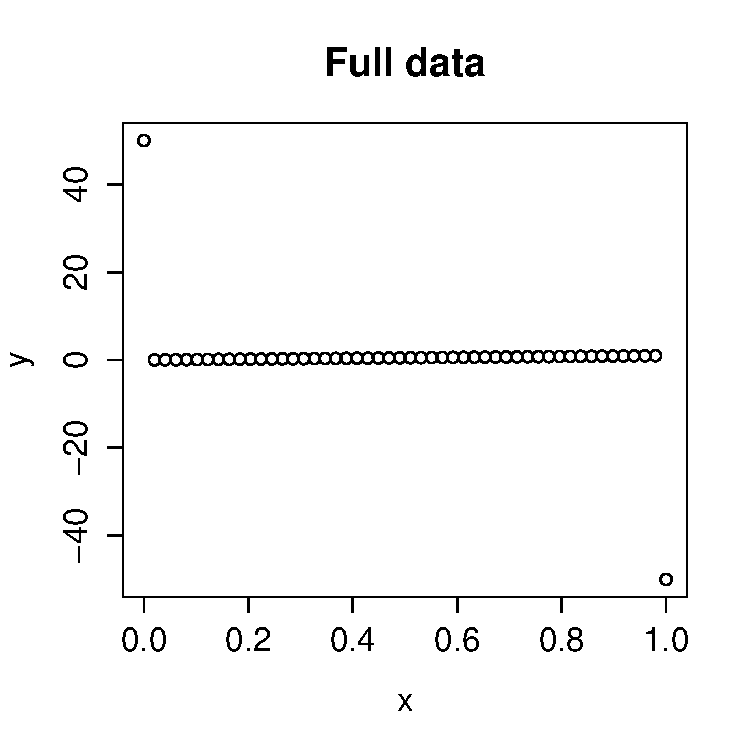
\includegraphics[width=0.45\textwidth]{figures/outlier-scatter.pdf}
    };
  \end{scope}
  \pause
  \begin{scope}[xshift=0.5\textwidth]
    \node [mybox] (box){
      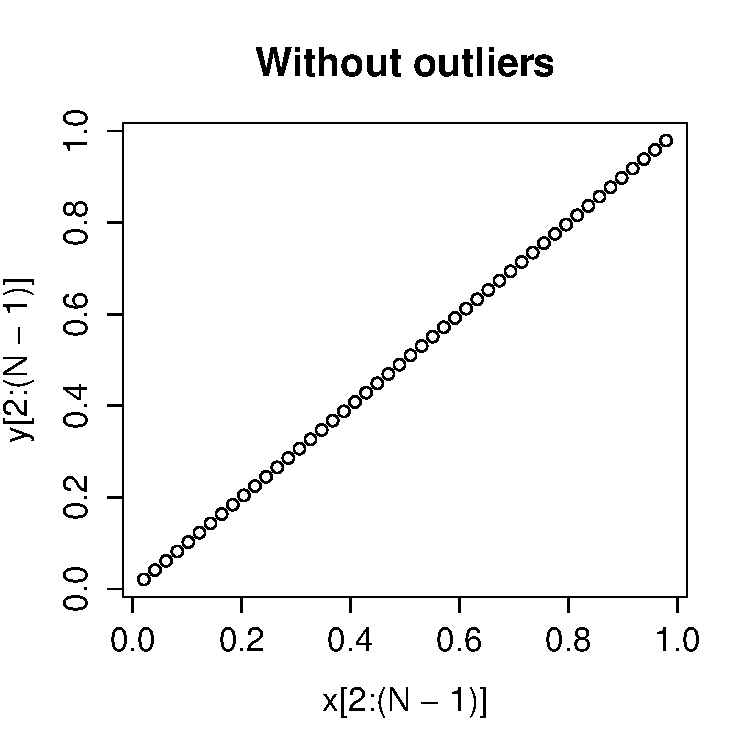
\includegraphics[width=0.45\textwidth]{figures/without-outliers.pdf}
    };
  \end{scope}
\end{tikzpicture}
\end{frame}

\begin{frame}{A version of the scientific method}
  \begin{center}
  \tikzstyle{block} = [rectangle, draw, fill=blue!20, 
                       text width=0.2\textwidth, text centered, rounded corners, minimum height=3em]
  \tikzstyle{line} = [draw, -latex', ultra thick]
  \tikzstyle{thin line} = [draw, -latex']
  \tikzstyle{cloud} = [draw, ellipse,fill=red!20,minimum height=2em]
    
  \begin{tikzpicture}[node distance = 0.3\textwidth]
    \footnotesize
    % Place nodes
    \node [block] at (0, 0) (hypothesis) {Hypothesis generation};
    \node [block] at (0.4\textwidth, 0) (infer) {Deduction and inference};
    \node [cloud] at (0.4\textwidth, -0.2\textwidth) (apply) {Application};
    \node [cloud] at (0.4\textwidth, +0.2\textwidth) (data) {Data};
    \node [block] at (0.8\textwidth, 0) (criticise) {Evaluation and criticism};
    % Draw edges
    \path [line] (hypothesis.east) -- (infer.west);
    \path [line] (infer.east) -- (criticise.west);
    \path [thin line] (infer.south) -- (apply.north);
    \path [thin line] (data.south) -- (infer.north);
    \path [thin line] (data.south east) -- (criticise.north west);
    \path [thin line] (hypothesis.north east) -- (data.south west);
    \path [thin line] (criticise.south west) -- (apply.north east);
    \draw[->, ultra thick] (criticise.south) .. controls (0.8\textwidth,-0.4\textwidth) and (0.0\textwidth,-0.4\textwidth) .. (hypothesis.south);
  \end{tikzpicture}
  \end{center}
\end{frame}

\begin{frame}{Many ML papers stop at evaluation}
  \begin{center}
  \tikzstyle{block} = [rectangle, draw, fill=blue!20, 
                       text width=0.2\textwidth, text centered, rounded corners, minimum height=3em]
  \tikzstyle{line} = [draw, -latex', ultra thick]
  \tikzstyle{thin line} = [draw, -latex']
  \tikzstyle{cloud} = [draw, ellipse,fill=red!20,minimum height=2em]
    
  \begin{tikzpicture}[node distance = 0.3\textwidth]
    \footnotesize
    % Place nodes
    \node [block] at (0, 0) (hypothesis) {Hypothesis generation};
    \node [block] at (0.4\textwidth, 0) (infer) {Deduction and inference};
    \node [cloud] at (0.4\textwidth, -0.2\textwidth) (apply) {Application};
    \node [cloud] at (0.4\textwidth, +0.2\textwidth) (data) {Data};
    \node [block] at (0.8\textwidth, 0) (criticise) {Evaluation and \dots};
    % Draw edges
    \path [line] (hypothesis.east) -- (infer.west);
    \path [line] (infer.east) -- (criticise.west);
    \path [thin line] (infer.south) -- (apply.north);
    \path [thin line] (data.south) -- (infer.north);
    \path [thin line] (data.south east) -- (criticise.north west);
    \path [thin line] (hypothesis.north east) -- (data.south west);
    \path [thin line] (criticise.south west) -- (apply.north east);
    \draw[->, dashed] (criticise.south) .. controls (0.8\textwidth,-0.4\textwidth) and (0.0\textwidth,-0.4\textwidth) .. (hypothesis.south);
  \end{tikzpicture}
  \end{center}
\end{frame}

\begin{frame}{Agenda}
  \begin{itemize}
  	\item Why I became interested in model criticism
    \vspace{\baselineskip}
    \item Review of frequentist and Bayesian theory
    \vspace{\baselineskip}
    \item A concern about calibration and a potential resolution
    \vspace{\baselineskip}
    \item An application of a nonparametric test to model criticism
    \vspace{\baselineskip}
    \item Discussion
  \end{itemize}
\end{frame}

\begin{frame}{My journey with model criticism}
  \begin{itemize}
    \item My previous research has involved automatic statistical model building
    \vspace{\baselineskip}
    \pause
    \item I wanted these model building systems to know when they had produced a model which was `obviously' wrong
    \vspace{\baselineskip}
    \pause
    \item On entering the literature I found a Bayesians vs frequentists debate that does not appear to have been resolved\dots
    \vspace{\baselineskip}
    \pause
    \item \dots and generally very little actionable advice on which method of model criticism to use and when
  \end{itemize}
\end{frame}

\begin{frame}{Is this model `correct'?}
  \begin{center}
  \begin{tikzpicture}
    \begin{scope}[yshift=0.0\textwidth]
    \node at (-0.25\textwidth, 0) {\includegraphics[width=0.5\textwidth]{figures/11-unemployment/11-unemployment_raw_data}};
    \node at (0.25\textwidth, 0) {\includegraphics[width=0.5\textwidth]{figures/11-unemployment/11-unemployment_all}};
    \end{scope}
    \pause
    \begin{scope}[yshift=-0.25\textwidth]
    \node at (-0.333\textwidth, 0) {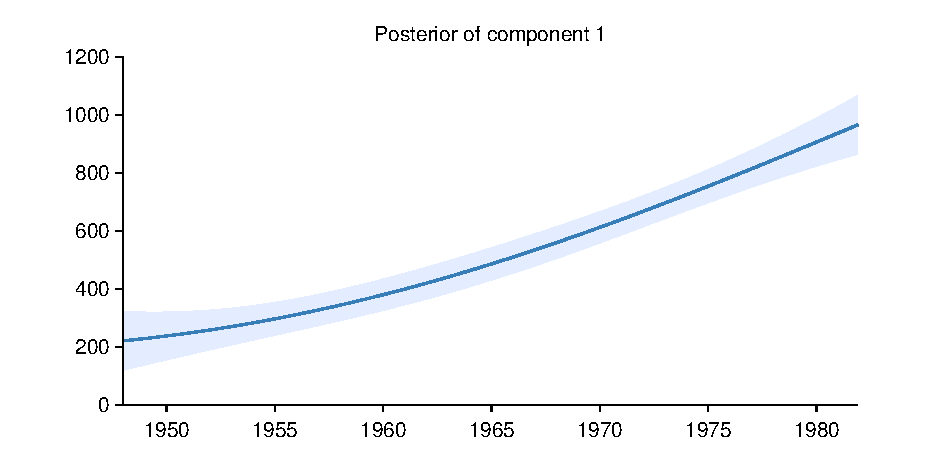
\includegraphics[width=0.3\textwidth]{figures/11-unemployment/11-unemployment_1}};
    \node at (0.0\textwidth, 0) {\includegraphics[width=0.3\textwidth]{figures/11-unemployment/11-unemployment_2}};
    \node at (0.333\textwidth, 0) {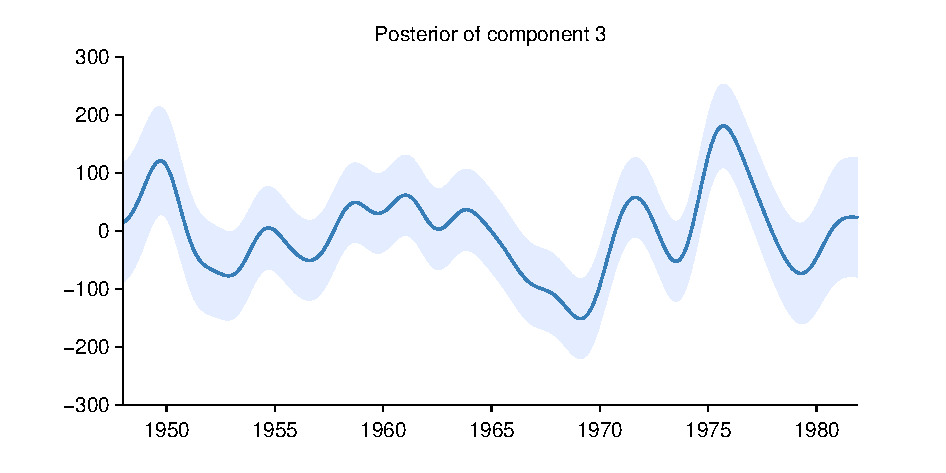
\includegraphics[width=0.3\textwidth]{figures/11-unemployment/11-unemployment_3}};
    \end{scope}
    \begin{scope}[yshift=-0.45\textwidth]
    \node at (-0.166666\textwidth, 0) {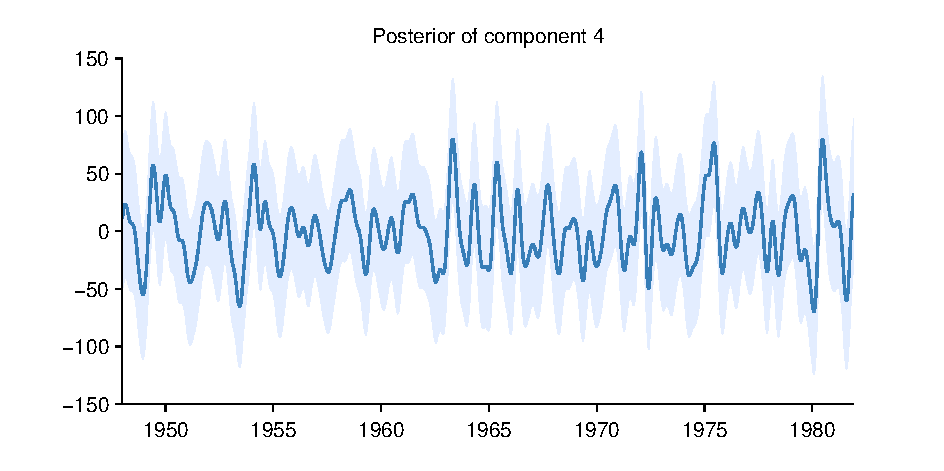
\includegraphics[width=0.3\textwidth]{figures/11-unemployment/11-unemployment_4}};
    \node at (0.166666\textwidth, 0) {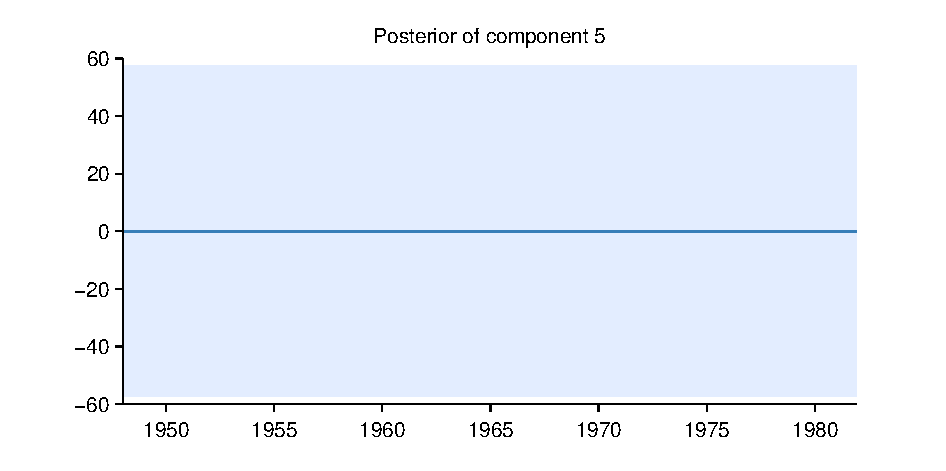
\includegraphics[width=0.3\textwidth]{figures/11-unemployment/11-unemployment_5}};
    \end{scope}
  \end{tikzpicture}
  \end{center}
\end{frame}

\begin{frame}{Frequentist model criticism}
  \begin{itemize}
    \item We suppose that our data are generated by some parametric model with unknown parameters
    \begin{itemize}
      \item $X \,|\, \theta \sim f(x\,|\,\theta)$
    \end{itemize}
    \vspace{\baselineskip}
    \pause
    \item We wish to test this null hypothesis and control the rate of false positives (Type I errors)
    \vspace{\baselineskip}
    \pause
    \item A typical method is to calculate a $p$-value which is a function of the data
    \vspace{\baselineskip}
    \pause
    \item A frequentist $p$-value is a random variable which has a uniform $[0,1]$ distribution under the null hypothesis
  \end{itemize}
\end{frame}

\begin{frame}{Frequentist model criticism}
  \begin{itemize}
    \item Constructing a $p$-value typically proceeds by choosing a statistic $T$ which is a function of the data
    \begin{itemize}
      \item The statistic is chosen such that large values are undesirable \eg outliers
    \end{itemize}
    \vspace{\baselineskip}
    \pause
    \item If $\theta$ were known then we could define $p$-values as
    \begin{itemize}
      \item $p(x_{\textrm{obs}}) = \mathbb{P}_{f(x\,|\,\theta)}(T(X) > T(x_{\textrm{obs}}))$
      \item \ie We will be suspicious of our model when $T(x_{\textrm{obs}})$ is large
    \end{itemize}
    \vspace{\baselineskip}
    \pause
    \item When $\theta$ is unknown a typical approach is to choose $T$ such that its distribution is independent of $\theta$
    \begin{itemize}
      \item These are called pivotal quantites
      \item Studentised residuals are an example of a pivotal quantity
    \end{itemize}
  \end{itemize}
\end{frame}

\begin{frame}{Maximum likelihood linear regression}
  \begin{itemize}
    \item Assume that outputs $y$ are linearly related to inputs $X$ plus independent Gaussian errors or noise $\varepsilon$
    \begin{itemize}
      \item $y = X\beta + \varepsilon$
      \item $\varepsilon \simiid \mathcal{N}(0, \sigma^2)$
    \end{itemize}
    \pause
    \vspace{\baselineskip}
    \item Maximum likelihood solution can be found analytically
    \begin{itemize}
      \item $\hat\beta = (X^{\textrm{T}}X)^{-1}X^{\textrm{T}}y$
      \item $\hat\sigma^2 = \|y - X \hat\beta\|^2 / n$
    \end{itemize}
    \pause
    \vspace{\baselineskip}
    \item Many assumptions to be tested before we believe these solutions
    \begin{itemize}
      \item \eg $X$ non-random, linearity, constant variance, Gaussianity, independent errors
    \end{itemize}
  \end{itemize}
\end{frame}

\begin{frame}{Outliers}
  \begin{itemize}
    \item Perhaps some of the errors are unexpectedly large?
    \pause
    \vspace{\baselineskip}
    \item We can check this by comparing $\hat\varepsilon = y - X\hat\beta$ to its expected distribution
    \pause
    \vspace{\baselineskip}
    \item Let $H = X(X^{\textrm{T}}X)^{-1}X^{\textrm{T}}$, then $\frac{\hat\varepsilon_i}{\hat\sigma\sqrt{1 - h_{ii}}}$ has a standard $t$-distribution when $\hat\sigma$ is the standard unbiased estimator of $\sigma$
    \pause
    \vspace{\baselineskip}
    \item These are the studentised residuals
    \begin{itemize}
      \item They are pivotal quantities since their distribution does not depend on $\beta$ or $\sigma$.
    \end{itemize}
  \end{itemize}
\end{frame}

\begin{frame}{Bayesian model criticism}
  \begin{itemize}
    \item The frequentist approach tests whether or not the data $x_{\textrm{obs}}$ could have been generated by the `model' $f(x\,|\,\theta)$ for any $\theta$
    \vspace{\baselineskip}
    \pause
    \item A more relevant null hypothesis for a Bayesian is that the data was generated from the prior predictive distribution
    \begin{itemize}
      \item Prior predictive just means the prior over data (as opposed to parameters)
    \end{itemize}
    \vspace{\baselineskip}
    \pause
    \item We could therefore compute prior predictive $p$-values
    \begin{itemize}
      \item $p_{\textrm{prior}}(x_{\textrm{obs}}) = \mathbb{P}_{f(x\,|\,\theta)\pi(\theta)}(T(X) > T(x_{\textrm{obs}}))$
      \item \cite{Box1980-ud}
    \end{itemize}
  \end{itemize}
\end{frame}

\begin{frame}{Prior predictive $p$-values}
  \begin{itemize}
    \item These $p$-values allow us to answer the question:
    \begin{itemize}
      \item Is some aspect of the data extreme given my prior assumptions?
    \end{itemize}
    \vspace{\baselineskip}
    \pause
    \item The statistic $T$ measures the way in which the data is extreme
    \vspace{\baselineskip}
    \pause
    \item Ill-defined when using improper priors 
    \vspace{\baselineskip}
    \pause
    \item Vague priors can lead to vague tests
    \begin{itemize}
      \item Probably best used when one really has a subjective prior or the model is not vague about the test statistic
    \end{itemize}
  \end{itemize}
\end{frame}

\begin{frame}{Example: Speed of light data}
  \begin{center}
    \begin{tikzpicture}[scale=1]
      \begin{scope}[xshift=0\textwidth]
        \node [mybox] (box){
          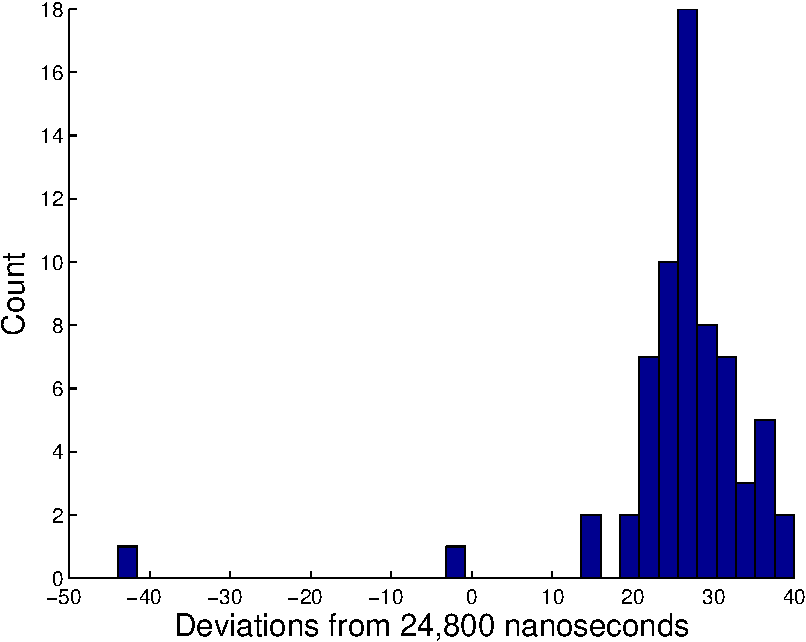
\includegraphics[width=0.45\textwidth]{figures/newcomb_hist.pdf}
        };
      \end{scope}
    \end{tikzpicture}
  \end{center}
  \begin{itemize}
    \pause
    \item Suppose we wish to fit a normal distribution to this data with vague priors on the mean and variance
    \vspace{\baselineskip}
    \pause
    \item We could test this assumption using skewness as the test statistic
    \pause
    \begin{itemize}
      \item Skewness = -4.5; $p$-value = tiny
    \end{itemize}
  \end{itemize}
\end{frame}

\begin{frame}{Posterior predictive $p$-values}
  \begin{itemize}
    \item Rubin \cite{Rubin1984-tw} instead proposed comparing statistics to their distribution under the posterior distribution
    \begin{itemize}
      \item $p_{\textrm{post}}(x_{\textrm{obs}}) = \mathbb{P}_{f(x\,|\,\theta)\pi(\theta\,|\,x_{\textrm{obs}})}(T(X) > T(x_{\textrm{obs}}))$
    \end{itemize}
    \vspace{\baselineskip}
    \pause
    \item These $p$-values allow us to answer the question:
    \begin{itemize}
      \item If I were to observe more data, would I be surprised if it was as extreme as the data I originally observed?
    \end{itemize}
    \vspace{\baselineskip}
    \pause
    \item One may be concerned about using the data twice
    \begin{itemize}
      \item The common retort is that the posterior predictive $p$-value is a well defined subjective probability statement and should be interpreted as such
    \end{itemize}
  \end{itemize}
\end{frame}

\begin{frame}{Example: Speed of light data again}
  \begin{itemize}
    \item Is the minimum value in the data surprising?
    \vspace{\baselineskip}
    \pause
    \item A prior predictive would be vague about this quantity
    \vspace{\baselineskip}
    \pause
    \item Instead we can test this by sampling data sets of the same size from the posterior, and recording their minima
    \pause
  \end{itemize}
  \begin{center}
    \begin{tikzpicture}[scale=1]
      \begin{scope}[xshift=0\textwidth]
        \node [mybox] (box){
          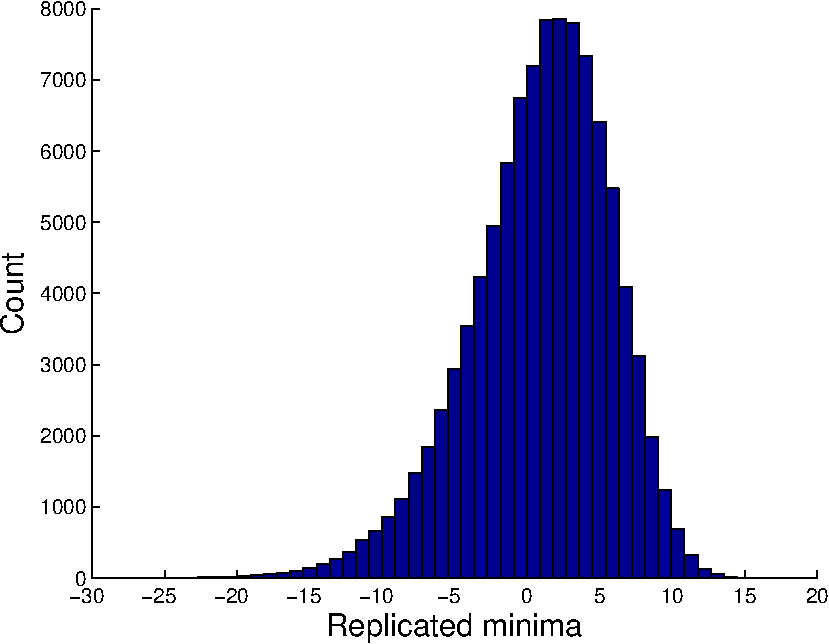
\includegraphics[width=0.45\textwidth]{figures/minima_hist.pdf}
        };
      \end{scope}
      \begin{scope}[xshift=0.5\textwidth]
        \node [mybox] (box){
          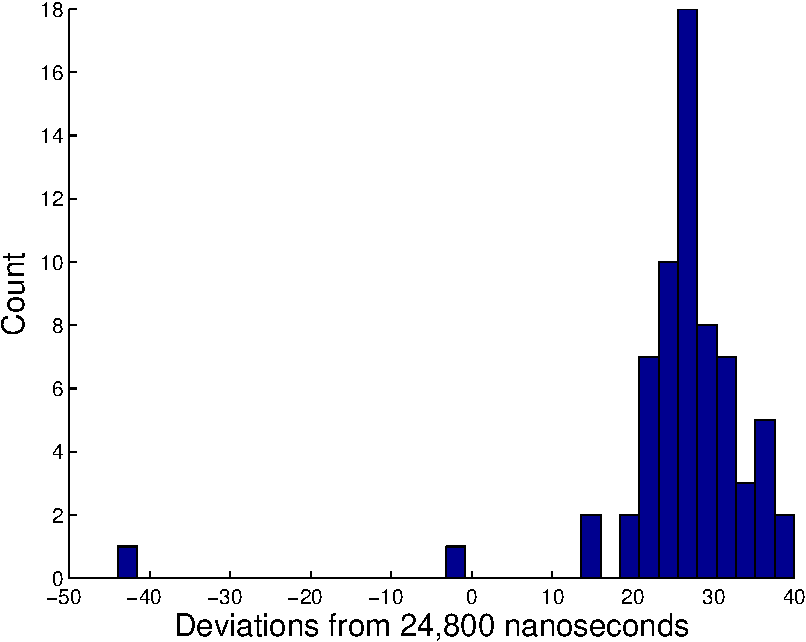
\includegraphics[width=0.45\textwidth]{figures/newcomb_hist.pdf}
        };
      \end{scope}
    \end{tikzpicture}
  \end{center}
\end{frame}

\begin{frame}{A problem of calibration}
  \begin{itemize}
    \item The Bayesian $p$-values defined thus far are not frequentist $p$-values
    \vspace{\baselineskip}
    \pause
    \item Alternatives were proposed by \cite{Bayarri1999-ty} and were shown to be asymptotically frequentist $p$-values by \cite{Robins2000-oz}
    \vspace{\baselineskip}
    \pause
    \item But maybe this isn't a problem --- perhaps we are confusing the use of the word `model'
    \begin{itemize}
      \item \textit{``If our goal is to check the model $f(x;\theta)$ rather than the prior $\pi(\theta)$, our procedures should perform adequately whatever the prior, including point-mass priors''} --- James Robins discussion of \cite{Bayarri1999-ty}
    \end{itemize}
  \end{itemize}
\end{frame}

\begin{frame}{Different tests for different goals}
  \begin{itemize}
    \item Frequentist $p$-values test an entire class of models
    \begin{itemize}
      \item The null hypothesis is that the data could have been generated by $f(x\,|\,\theta)$ for some $\theta$
    \end{itemize}
    \vspace{\baselineskip}
    \pause
    \item Prior predictive $p$-values test a particular prior distribution
    \begin{itemize}
      \item The null hypothesis is that the data could have been generated from the prior distribution
    \end{itemize}
    \vspace{\baselineskip}
    \pause
    \item Posterior predictive $p$-values use the data twice so require a different interpretation
    \begin{itemize}
      \item Can be interpreted literally as the probability of a future data set being more extreme than the one just observed
    \end{itemize}
    \vspace{\baselineskip}
    \pause
    \item Can also use held out data to test posterior distributions
  \end{itemize}
\end{frame}

\begin{frame}{How do we choose the test statistic?}
  \begin{itemize}
    \item All of the tests so far have required a statistic by which one measures if the data is extreme
    \vspace{\baselineskip}
    \pause
    \item We could apply a battery of statistics to every problem
    \begin{itemize}
      \item Without understanding dependencies between all statistics multiple comparisons adjustments will become highly conservative
    \end{itemize}
    \vspace{\baselineskip}
    \pause
    \item Can we instead define a statistic in high level terms, and then compute the statistic which most demonstrates any discrepancy?
    \pause
    \begin{itemize}
      \item And will we be able to interpret this statistic?
    \end{itemize}
  \end{itemize}
\end{frame}

\begin{frame}{Maximum mean discrepancy two sample tests}
  \begin{itemize}
    \item Suppose we have samples $x \simiid p$ and $y \simiid q$ and we wish to test the hypothesis $p = q$
    \vspace{\baselineskip}
    \pause
    \item Define $\textrm{MMD}(\mathcal{F},p,q) = \sup_{f \in \mathcal{F}}(\mathbb{E}_{x\sim p}[f(x)] - \mathbb{E}_{y\sim q}[f(y)])$ where $\mathcal{F}$ is a reproducing kernel Hilbert space (RKHS) with kernel $k$
    \vspace{\baselineskip}
    \pause
    \item The function attaining this supremum can be computed analytically
    \begin{itemize}
      \item $f(x) = \mathbb{E}_{x'\sim p}[k(x,x')] - \mathbb{E}_{x'\sim q}[k(x,x')]$
    \end{itemize}
    \vspace{\baselineskip}
    \pause
    \item Substituting and squaring:
    \begin{itemize}
		\item $\textrm{MMD}^2(\mathcal{F},p,q) = \mathbb{E}_{x,x'\sim p}[k(x,x')] + 2\mathbb{E}_{x\sim p,y\sim q}[k(x,y)] + \mathbb{E}_{y,y'\sim q}[k(y,y')]$
	\end{itemize}
  \end{itemize}
\end{frame}

\begin{frame}{Empirical estimation}
  \begin{itemize}
    \item We can estimate these expectations from finite samples
    \begin{itemize}
      \item $\textrm{MMD}_b^2(\mathcal{F},X,Y) = \frac{1}{m^2}\sum_{i,j=1}^{m}k(x_i,x_j) - \frac{2}{mn}\sum_{i,j=1}^{m,n}k(x_i,y_j) + \frac{1}{n^2}\sum_{i,j=1}^{n}k(y_i,y_j)$
      \item $\hat{f}(x) = \frac{1}{m}\sum_{i=1}^{m}k(x,x_i) - \frac{1}{n}\sum_{i=1}^{n}k(x,y_i)$
    \end{itemize}
    \vspace{\baselineskip}
    \pause
    \item The empirical witness function is just the difference of two kernel density estimates
    \vspace{\baselineskip}
    \pause
    \item We can estimate the null distribution of the MMD statistic by a bootstrap procedure
    \begin{itemize}
      \item It is an example of a permutation test
    \end{itemize}
  \end{itemize}
\end{frame}

\begin{frame}{Application to model checking}
  \begin{itemize}
    \item Need to make some simplifying assumptions
    \begin{itemize}
      \item Data $y$ are generated $\iid$ from some distribution $q$
      \item We make a point estimate of $q$ which we denote $p$
    \end{itemize}
    \vspace{\baselineskip}
    \pause
    \item The hypothesis that $p = q$ is now the hypothesis that the model is correct
    \vspace{\baselineskip}
    \pause
    \item We can generate samples from $p$ and then perform a two sample test
  \end{itemize}
\end{frame}

\begin{frame}{Example: Speed of light data again (again)}
  \begin{center}
  \begin{tabular}{cc}
    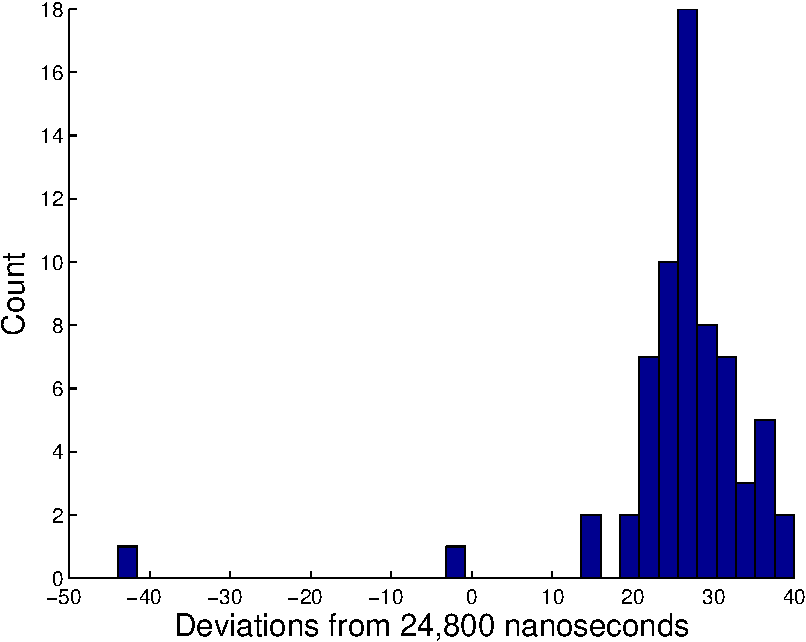
\includegraphics[width=0.435\textwidth]{figures/newcomb_hist} &
    \pause
    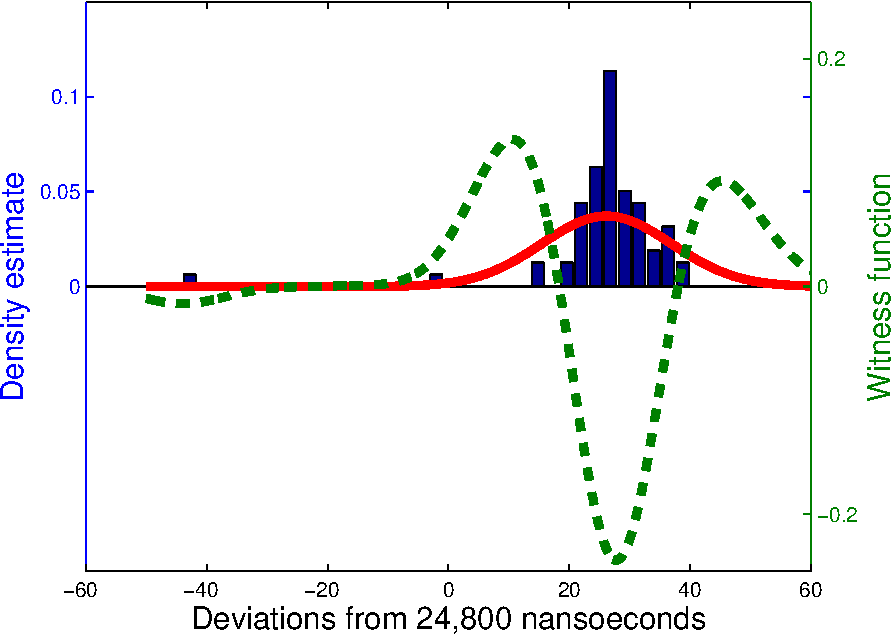
\includegraphics[width=0.48\textwidth]{figures/newcomb_witness_1}
  \end{tabular}
  \end{center}
  \pause
  \begin{center}
    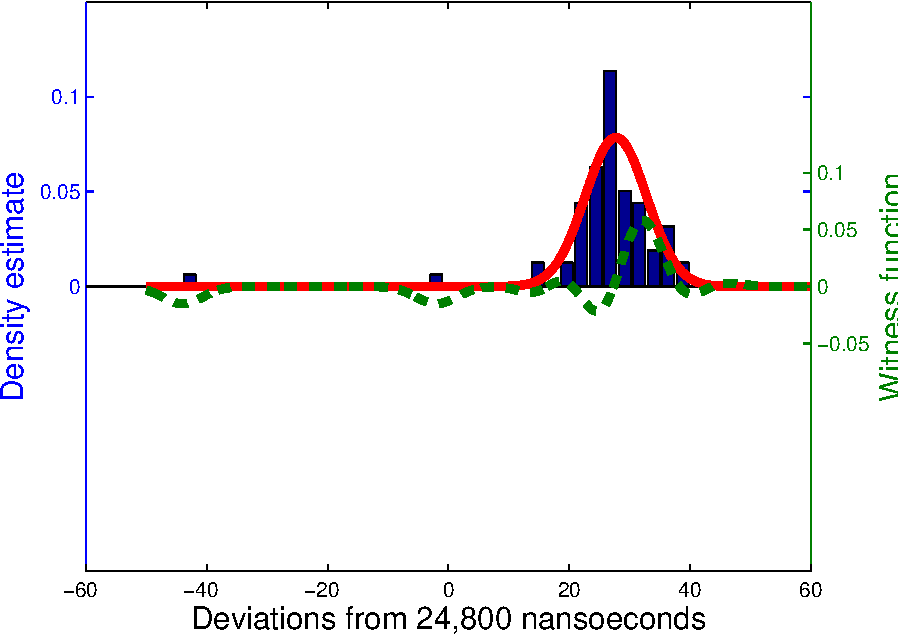
\includegraphics[width=0.48\textwidth]{figures/newcomb_witness_2}
  \end{center}
\end{frame}

\begin{frame}{What happens in high dimensions?}
  \begin{itemize}
    \item Interpretability of test comes from interpretation of witness function as difference of kernel density estimates
    \vspace{\baselineskip}
    \pause
    \item Kernel density estimation is high variance in high dimensions and will likely be uninterpretable
    \vspace{\baselineskip}
    \pause
    \item Potential solution: Include dimensionality reduction as part of the test statistic
    \begin{itemize}
      \item $\frac{1}{m^2}\sum_{i,j=1}^{m}k(x_i^{\textrm{PCA}},x_j^{\textrm{PCA}}) - \frac{2}{mn}\sum_{i,j=1}^{m,n}k(x_i^{\textrm{PCA}},y_j^{\textrm{PCA}}) + \frac{1}{n^2}\sum_{i,j=1}^{n}k(y_i^{\textrm{PCA}},y_j^{\textrm{PCA}})$
    \end{itemize}
  \end{itemize}
\end{frame}

\begin{frame}{What happens in high dimensions?}
  \begin{center}
  \begin{tabular}{cc}
    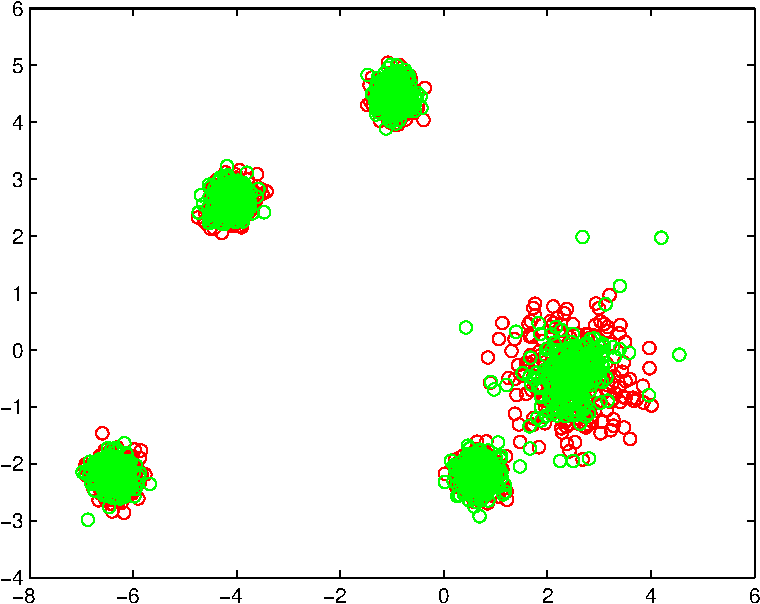
\includegraphics[width=0.48\textwidth]{figures/high_mog_pca} &
    \pause
    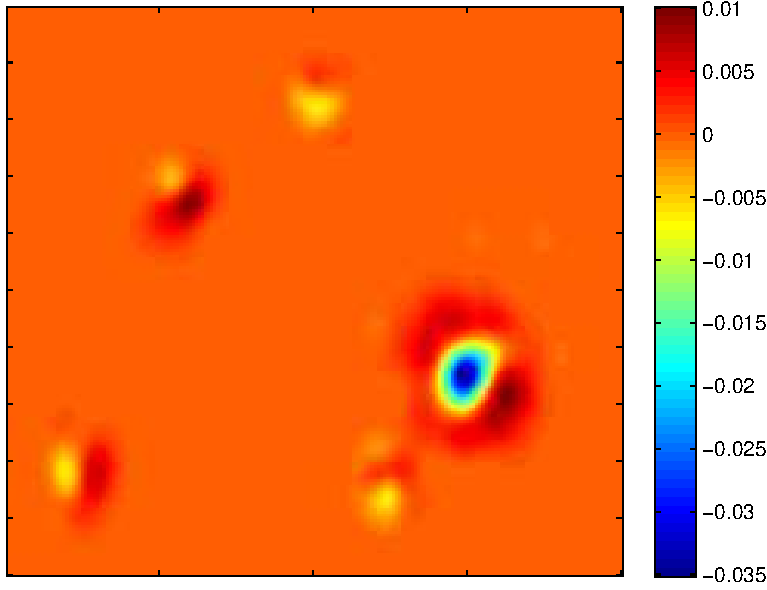
\includegraphics[width=0.48\textwidth]{figures/high_mog_witness}
  \end{tabular}
  \end{center}
  \pause
  \begin{itemize}
    \item Estimated $p$-value of 0.05
  \end{itemize}
\end{frame}

\begin{frame}{What do neural networks dream about?}
  \begin{itemize}
    \item Various versions of deep belief networks have been trained to produce generative models of MNIST handwritten digits
    \vspace{\baselineskip}
    \pause
    \item Samples from these models certainly look like digits, but what aspects of the distribution over handwritten digits do these models not capture?
  \end{itemize}
\end{frame}

\begin{frame}{An RBM trained on MNIST}
  \begin{center}
  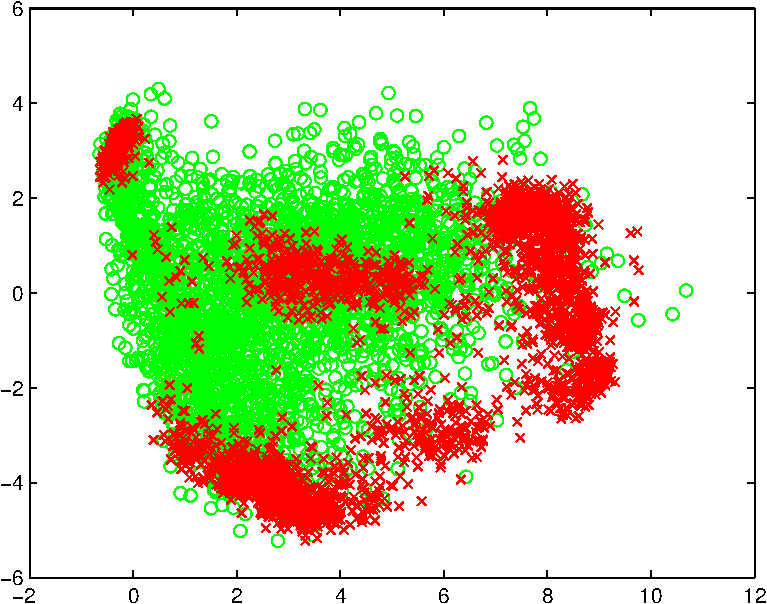
\includegraphics[width=0.4\textwidth]{figures/rbm_pca}
  \end{center}
  \pause
  \begin{center}
  \begin{tabular}{cc}
    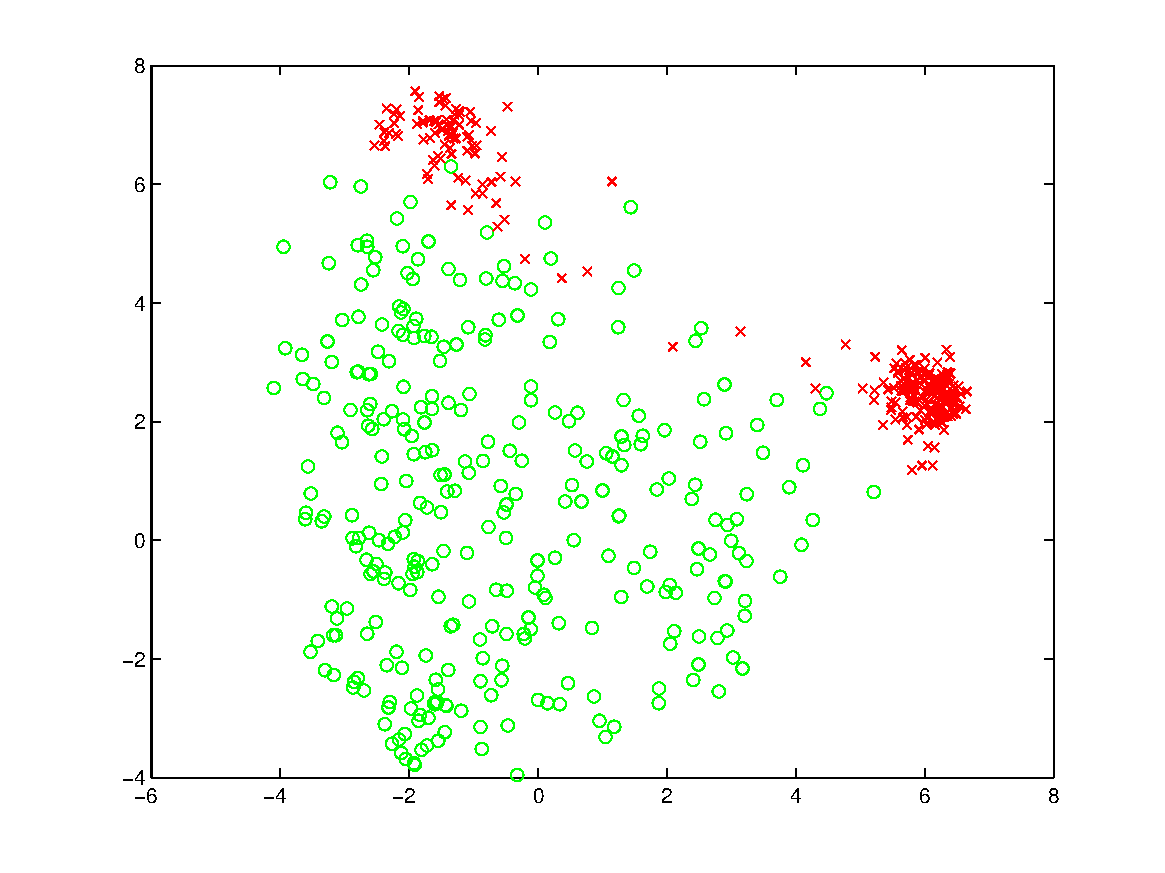
\includegraphics[width=0.4\textwidth]{figures/rbm_0_pca} & 
    \pause
    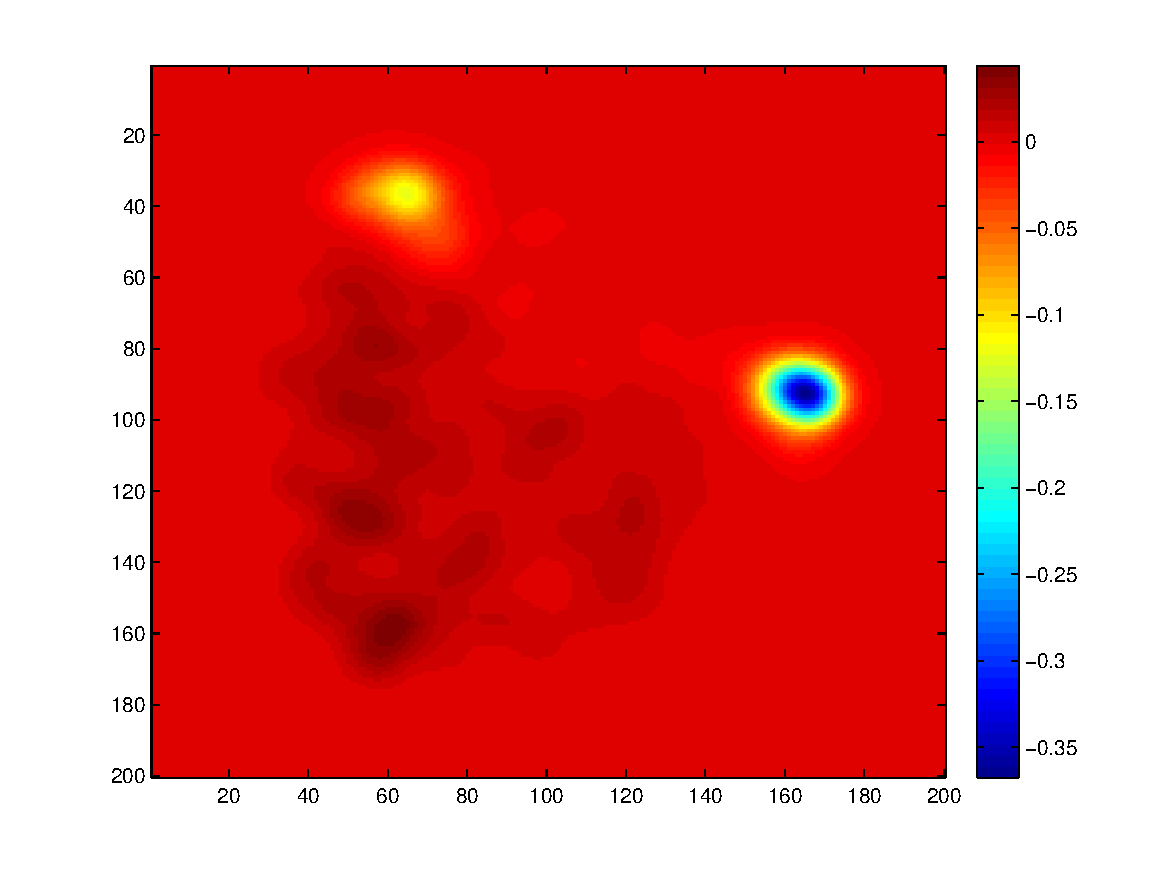
\includegraphics[width=0.4\textwidth]{figures/rbm_0_witness}
  \end{tabular}
  \end{center}
\end{frame}

\begin{frame}{What do neural networks dream about?}
  \begin{center}
    \begin{tabular}{ccc}
      Real digits & $\,$ & 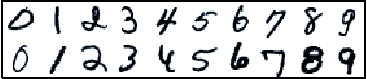
\includegraphics[width=0.48\textwidth]{figures/many_rbm_cond_witness_peaks} \\
      \pause
      Witness fn troughs : RBM & $\,$ & 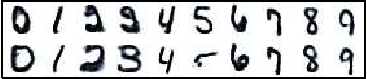
\includegraphics[width=0.48\textwidth]{figures/rbm_witness_troughs} \\
      \pause
      Witness fn troughs : RBMs & $\,$ & 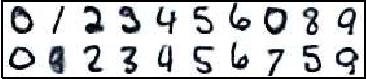
\includegraphics[width=0.48\textwidth]{figures/many_rbm_cond_witness_troughs} \\
      \pause
      Witness fn troughs : DBN & $\,$ & 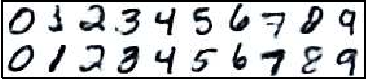
\includegraphics[width=0.48\textwidth]{figures/dbn_ft_cond_witness_troughs} \\
    \end{tabular}
  \end{center}
\end{frame}

\begin{frame}{Why have I not mentioned power?}
  \begin{itemize}
    \item Quantification of power requires specification of an explicit alternative model or hypothesis
    \vspace{\baselineskip}
    \pause
    \item ``Model criticism \dots is intended as an open-minded phase of investigation
to identify any problems with the model. Formulation of explicit alternatives
comes after the model criticism phase has identified some problems.'' \cite{OHagan2003-bc}
    \vspace{\baselineskip}
    \pause
    \item I'm not sure anymore that alternative free hypothesis tests are the correct way to think about model criticism
    \begin{itemize}
      \item Some effort should be made to characterise the alternative hypotheses for which certain tests have high power
    \end{itemize}
  \end{itemize}
\end{frame}

\begin{frame}{Future work}
  \begin{itemize}
    \item Can we usefully characterise the types of alternative models for which MMD tests have high power?
    \begin{itemize}
      \pause
      \item Using different kernels will identify different types of discrepancy
      \pause
      \item This characterisation probably already in the literature 
    \end{itemize}
    \vspace{\baselineskip}
    \pause
    \item Could these alternatives be usefully understood as specific nonparametric models by exploiting the connections between RKHSs and Gaussian processes?
  \end{itemize}
\end{frame}

\begin{frame}{Discussion}
  \begin{itemize}
    \item Box advocated for model criticism to be part of the loop of the scientific process\dots
    \begin{itemize}
      \item Probabilistic version of falsification
    \end{itemize}
    \vspace{\baselineskip}
    \pause
    \item \dots but should we just be estimating the utility of a model?
    \vspace{\baselineskip}
    \pause
    \item Perhaps we should be using model criticism to estimate the utility of expanding a model?
    \begin{itemize}
      \item They are often much cheaper to compute (thinking and computing time) than performing inference in an expanded model class
    \end{itemize}
    \vspace{\baselineskip}
    \pause
    \item What are other forms of model criticism that are widely applicable and can help identify the nature of discrepancies between model and data in highly complicated systems
  \end{itemize}
\end{frame}

{
\section{References}
\section{Extended Bibliography}
\tiny
\begin{frame}[allowframebreaks,plain]
  \frametitle{References}
  \bibliography{library}
  \bibliographystyle{alpha}
\end{frame}
}

\begin{frame}{Appendix}
\end{frame}

\begin{frame}{Is cross validation enough?}
  \begin{itemize}
    \item Machine learning is typically concerned with predictive accuracy\dots
    \vspace{\baselineskip}
    \pause
    \item \dots which can be estimated by cross validation
  \end{itemize}
  \begin{center}
    \begin{tabular}{|l|c|}
      \hline
      Algorithm & CV error (standard error) \\
      \hline
      Linear regression & 4.8 (1.3) \\
      Theil--Sen estimator & 2.0 (1.4) \\
      \hline
    \end{tabular}
  \end{center}
  \pause
  \begin{itemize}
    \item So we're fine, right?
  \end{itemize}
\end{frame}

\begin{frame}{Is cross validation enough?}
  \uncover<1->{
  \begin{itemize}
    \item Let's try some new data
  \end{itemize}
  }
  \only<2,3>{
  \begin{center}
    \begin{tabular}{|l|c|}
      \hline
      Algorithm & CV error (standard error) \\
      \hline
      Linear regression & 2.0 (0.1) \\
      Theil--Sen estimator & 1.3 (0.2) \\
      \hline
    \end{tabular}
  \end{center}
  }
  \only<3>{
  \begin{itemize}
    \item So outliers again?
  \end{itemize}
  }
  \uncover<4->{
  \begin{center}
    \begin{tabular}{|l|c|}
      \hline
      Algorithm & CV error (standard error) \\
      \hline
      Linear regression & 2.0 (0.1) \\
      Theil--Sen estimator & 1.3 (0.2) \\
      5 nearest neighbours & 0.1 (0.01) \\
      \hline
    \end{tabular}
  \end{center}
  }
  \uncover<5->{
  \begin{itemize}
    \item When I said outliers I actually meant non-linearity
  \end{itemize}
  }
  \uncover<6->{
    \begin{center}
      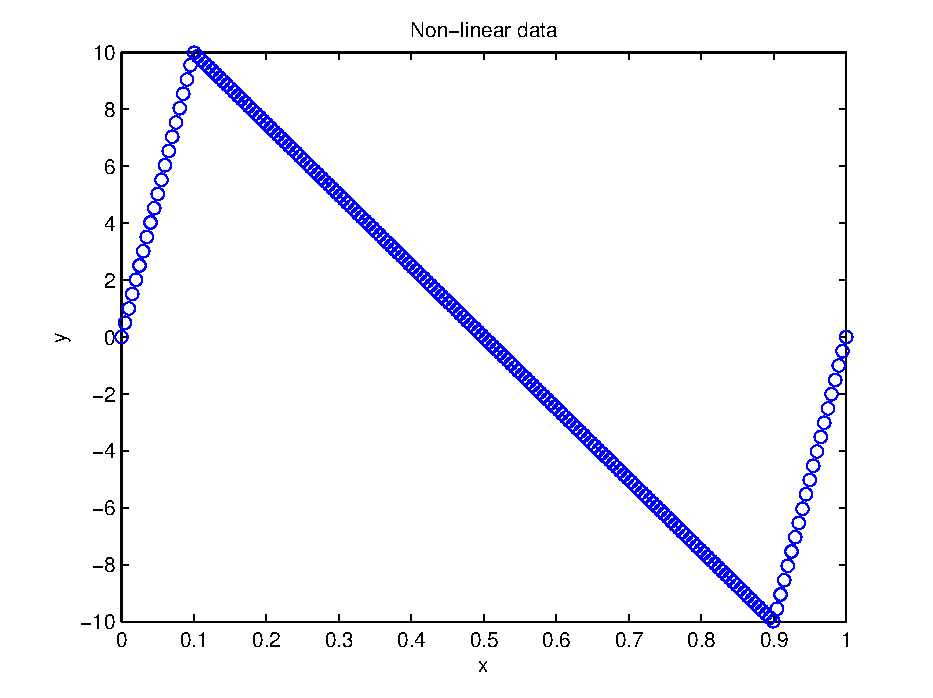
\includegraphics[width=0.45\textwidth]{figures/non-linear.pdf}
    \end{center}
  }
\end{frame}

\begin{frame}{Is being Bayesian enough?}
  \begin{itemize}
    \item Why not just do all inference in a super model that contains everything we could ever possibly believe?
    \pause
    \begin{itemize}
      \item And then \eg estimate the utility of smaller models for certain tasks
    \end{itemize}
    \vspace{\baselineskip}
    \pause
    \item How long did you spend coding your last inference scheme?
    \begin{itemize}
      \item Or have you ever got probabilistic programming to work in a non-trivial model?
    \end{itemize}
    \vspace{\baselineskip}
    \pause
    \item Model criticism / checking gives us tools to explore potential inadequacies of a method\dots
    \begin{itemize}
       \item \dots without having to implement inference for every expanded method we can think of
     \end{itemize}
  \end{itemize}
\end{frame}

\begin{frame}{Discrepancy $p$-values}
  \begin{itemize}
    \item Gelman et alia \cite{Gelman1996-ez} proposed generalising the statistic $T(x)$ of posterior predictive $p$-values to a discrepancy measure $d(x, \theta)$ which depends on the parameters $\theta$ of the model
    \vspace{\baselineskip}
    \pause
    \item The observed discrepancy is again compared to the posterior predictive distribution
    \vspace{\baselineskip}
    \pause
    \item $p_{\textrm{dis}}(x_{\textrm{obs}}) = \mathbb{P}(d(X,\theta) \geq d(x_{\textrm{obs}},\theta)\,|\,x_{\textrm{obs}})$
    \vspace{\baselineskip}
    \pause
    \item Can be estimated using samples of the joint posterior distribution of $(X, \theta)$ \eg from MCMC
  \end{itemize}
\end{frame}

\begin{frame}{Example: Forecasting U.S.\ elections}
  \begin{itemize}
    \item Copied without permission from Gelman, A. et al. Bayesian Data Analysis, Third Edition. (Taylor \& Francis, 2013)
    \vspace{\baselineskip}
    \item Fitting a linear model to proportion of votes for Democrats by state for 11 presidential elections
  \end{itemize}
  \begin{center}
    \begin{tikzpicture}[scale=1]
      \begin{scope}[xshift=0\textwidth]
        \node [mybox] (box){
          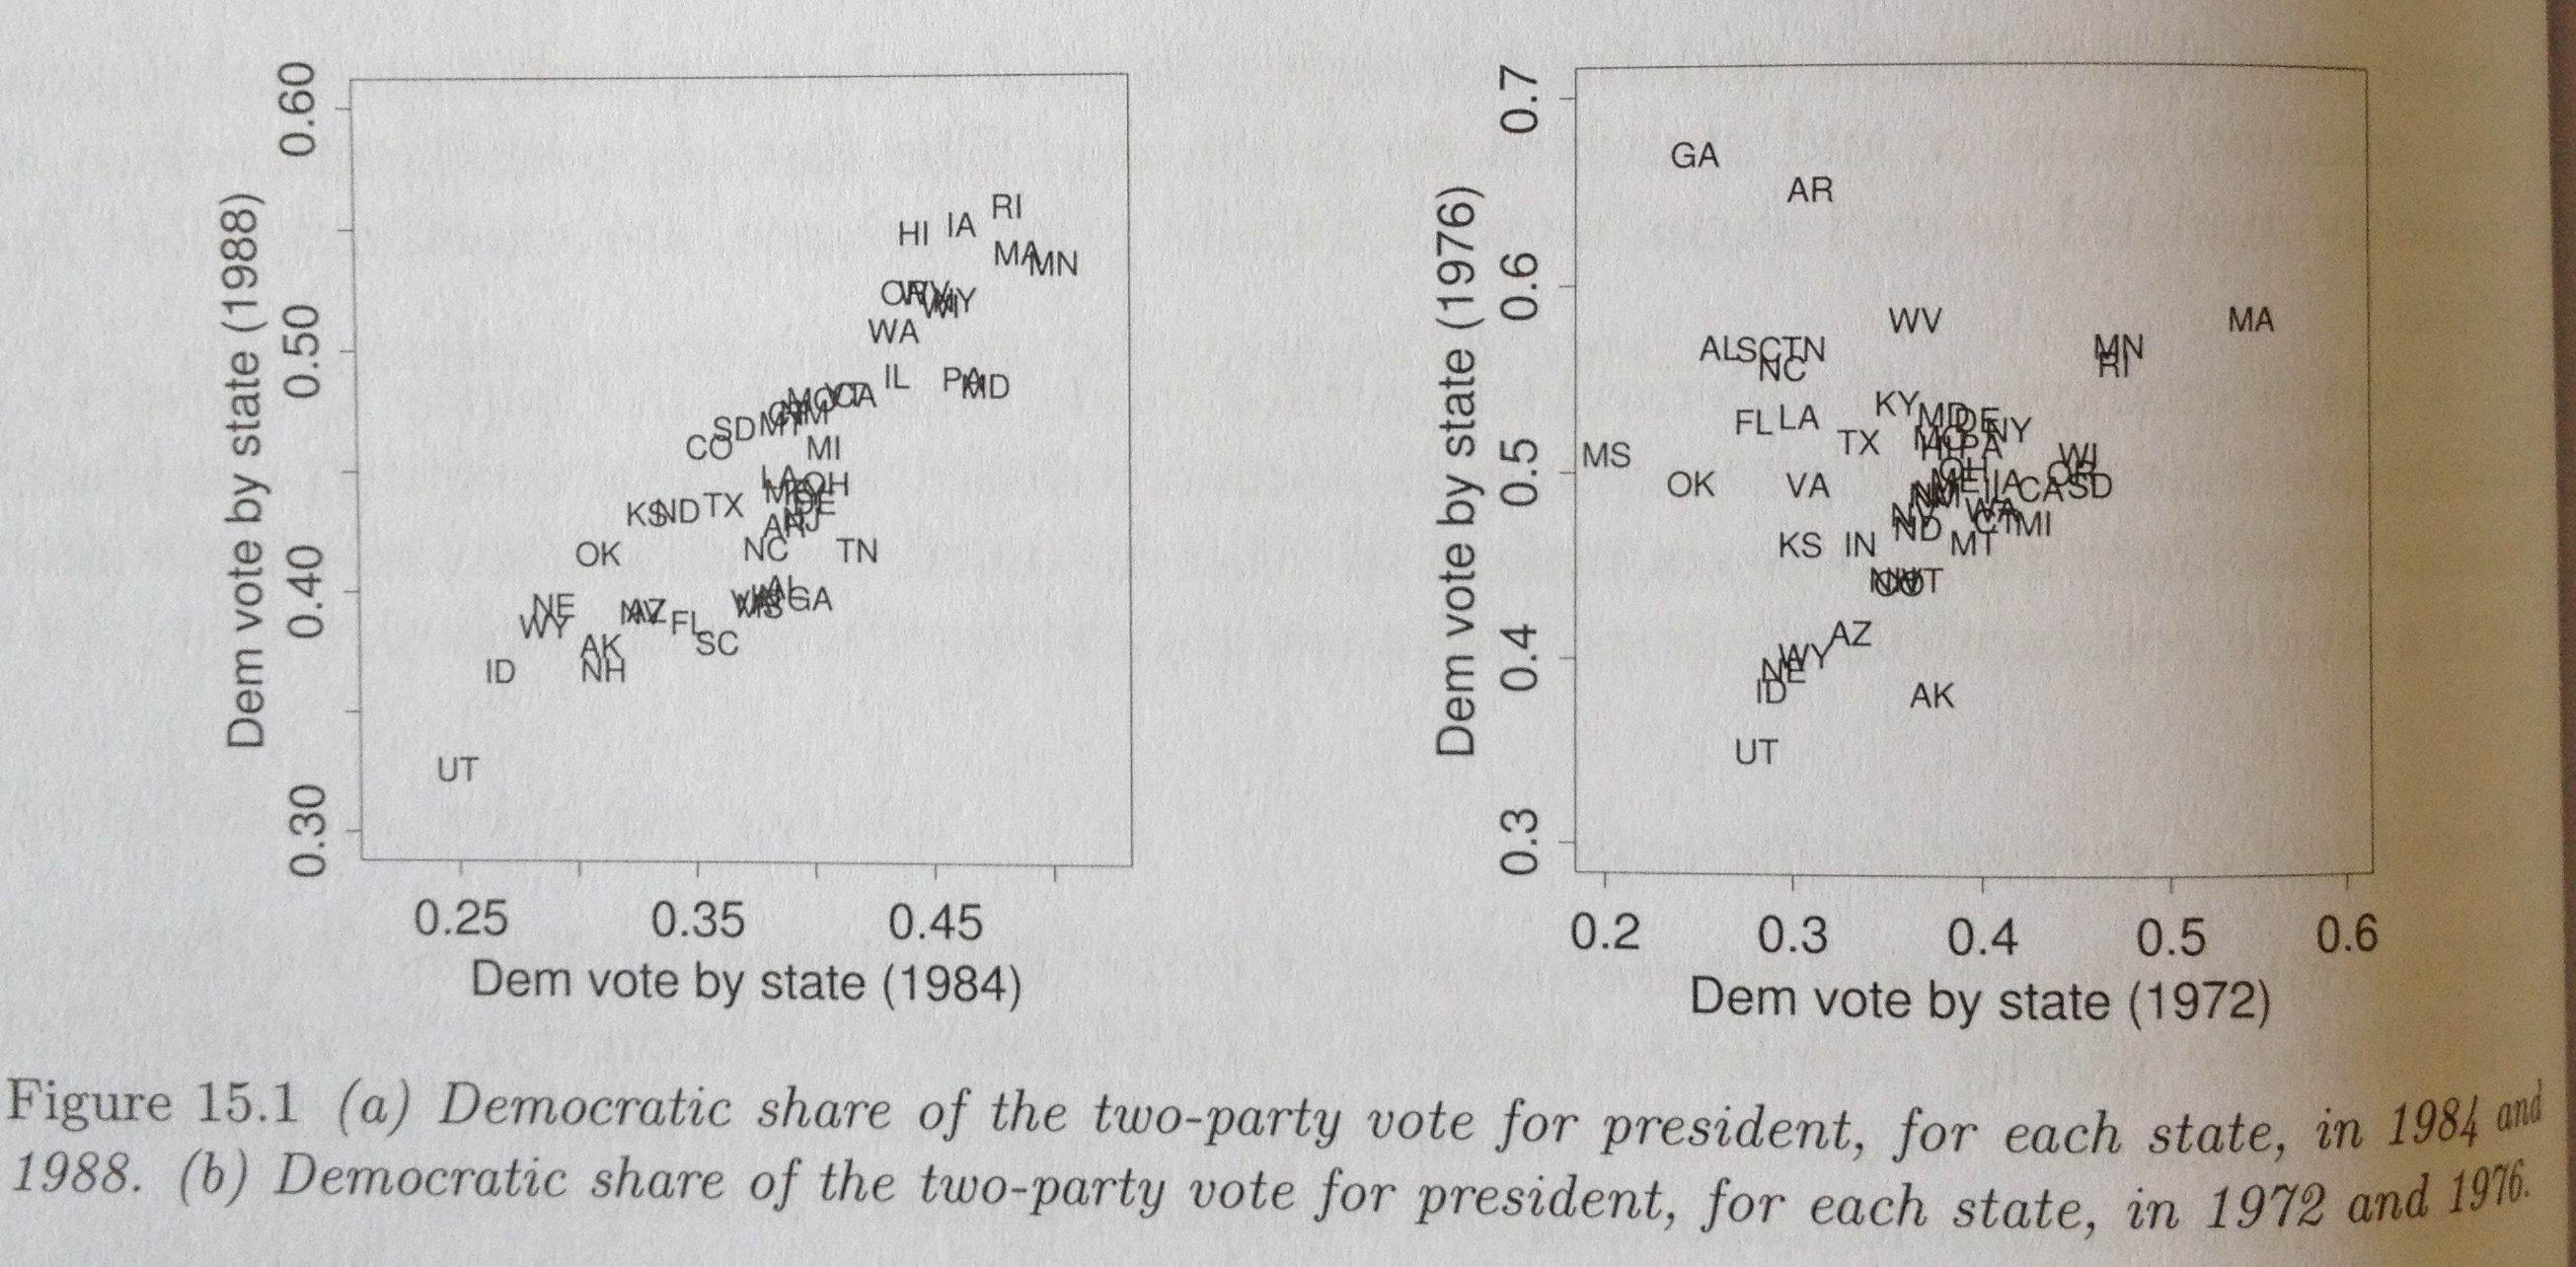
\includegraphics[width=0.8\textwidth]{figures/linear.jpg}
        };
      \end{scope}
    \end{tikzpicture}
  \end{center}
\end{frame}

\begin{frame}{Example: Forecasting U.S.\ elections}
  \begin{center}
    \begin{tikzpicture}[scale=1]
      \begin{scope}[xshift=0\textwidth]
        \node [mybox] (box){
          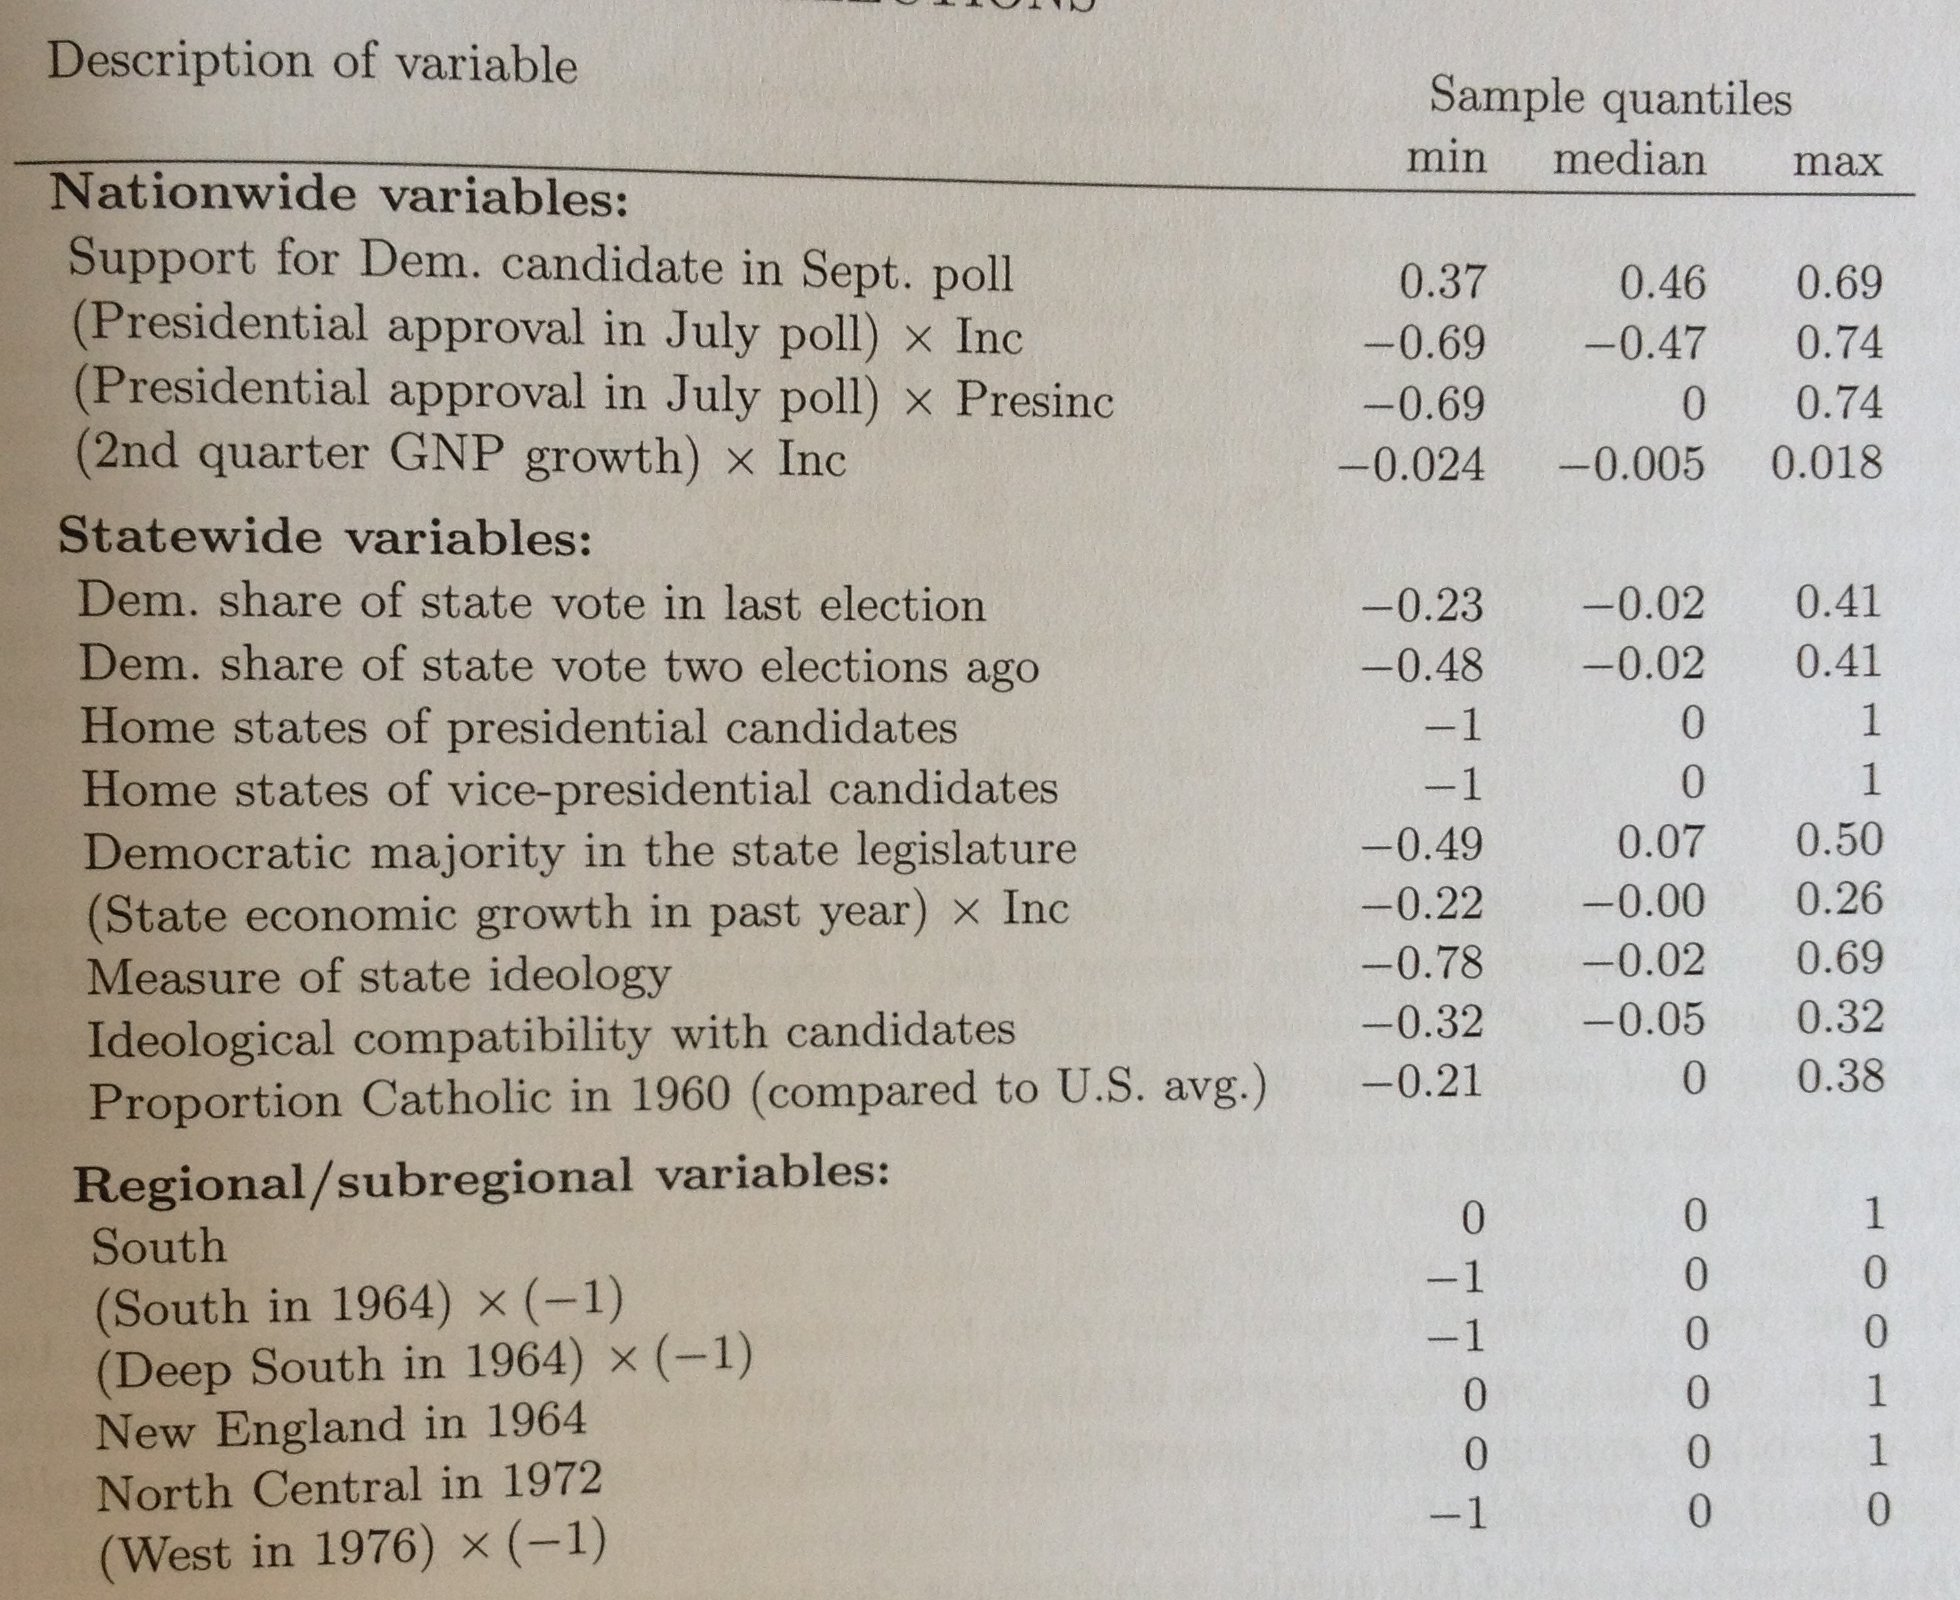
\includegraphics[width=0.8\textwidth]{figures/variables.jpg}
        };
      \end{scope}
    \end{tikzpicture}
  \end{center}
\end{frame}

\begin{frame}{Example: Forecasting U.S.\ elections}
  \begin{itemize}
    \item Linear model assumes that each (input, output) tuple is exchangeable
    \vspace{\baselineskip}
    \pause
    \item This ignores any correlation between states in a particular year due to nationwide swings in voting
    \vspace{\baselineskip}
    \pause
    \item We can construct a test staistic that can test for this correlation
    \begin{itemize}
      \item For each year compute the average error of the prediction in each state
      \item Compute the root mean square of these averageerrors over the 11 years
    \end{itemize}
  \end{itemize}
\end{frame}

\begin{frame}{Example: Forecasting U.S.\ elections}
  \begin{center}
    \begin{tikzpicture}[scale=1]
      \begin{scope}[xshift=0\textwidth]
        \node [mybox] (box){
          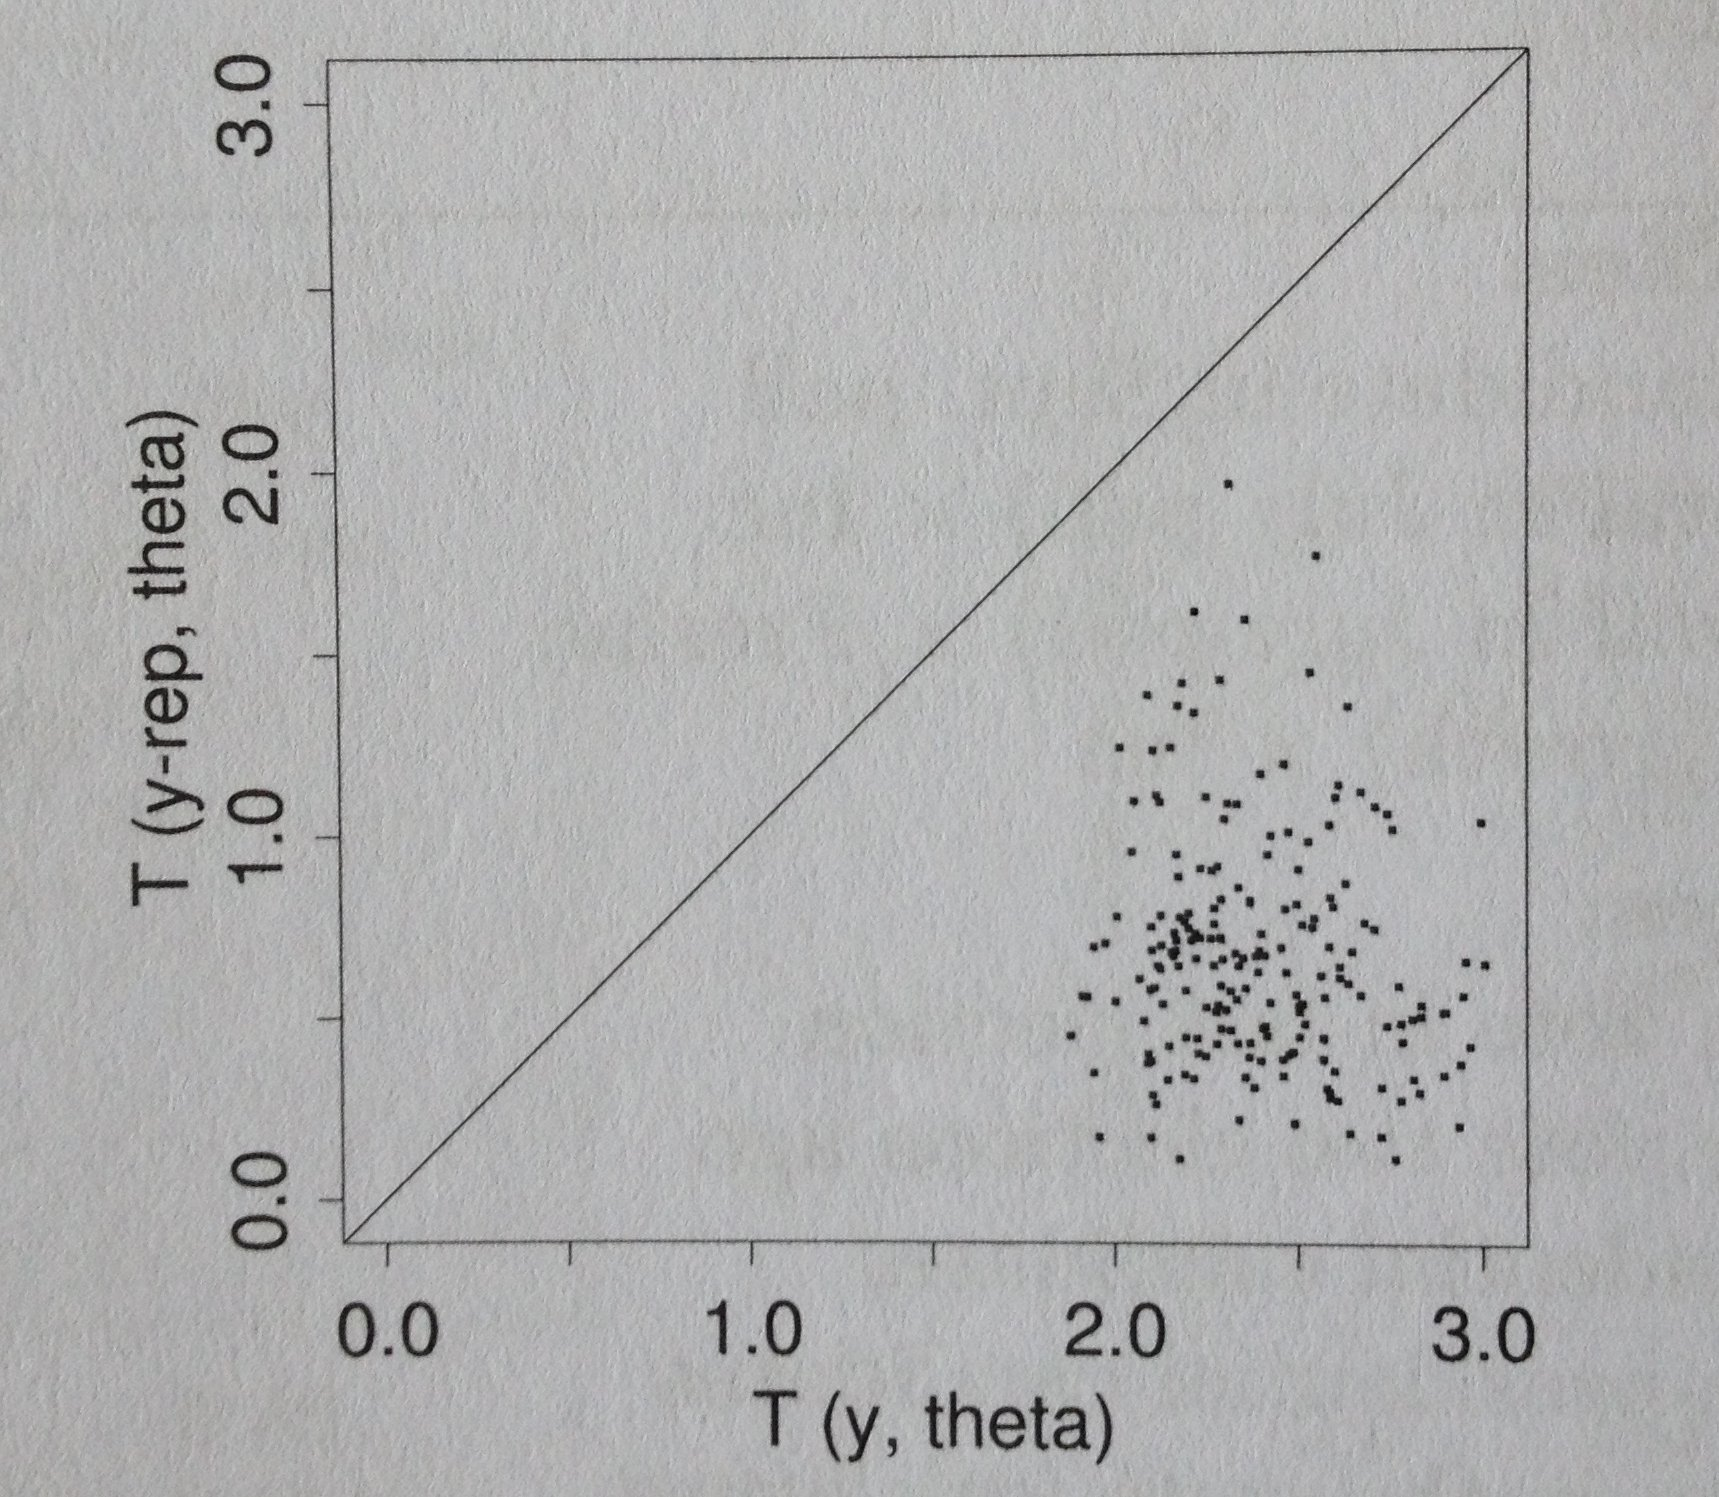
\includegraphics[width=0.8\textwidth]{figures/model_check.jpg}
        };
      \end{scope}
    \end{tikzpicture}
  \end{center}
\end{frame}

\begin{frame}{Example: Forecasting U.S.\ elections}
  \begin{itemize}
    \item The posterior distribution underestimates the test statistic
    \vspace{\baselineskip}
    \pause
    \item The practical consequence of this is that the model will give overly precise predictions of national election results
    \vspace{\baselineskip}
    \pause
    \item The model can be improved by adding indicator variables for each year
    \begin{itemize}
      \item Can also include year $\times$ region features to capture regional voting swings
    \end{itemize}
  \end{itemize}
\end{frame}

\begin{frame}{Model criticism for Gaussian processes}
  \begin{itemize}
    \item Suppose that $y_i \sim f(x_i) + \varepsilon_i$ where
    \begin{itemize}
      \item $f \sim \mathcal{GP}(0, k)$
      \item $\varepsilon \simiid \mathcal{N}(0, \sigma^2)$
    \end{itemize}
    \vspace{\baselineskip}
    \pause
    \item We might be interested in testing the residuals
    \begin{itemize}
      \pause
      \item We can construct a discrepancy measure based on some function of $y_i - f(x_i)$
      \pause
      \item A posterior predictive check would then correspond to comparing some function of the prior and posterior of $\varepsilon$
    \end{itemize}
    \vspace{\baselineskip}
    \pause
    \item Similarly, we could construct discrepancies based on $y_i - \varepsilon_i$
    \begin{itemize}
      \pause
      \item This amounts to comparing the prior and posterior of $f$
    \end{itemize}
  \end{itemize}
\end{frame}

\begin{frame}{Example: Is this model `correct'?}
\newcommand{\wmgd}{0.5\columnwidth}
\newcommand{\hmgd}{3.0cm}
\newcommand{\mdrd}{figures/11-unemployment}
\newcommand{\mbm}{\hspace{-0.3cm}}
\begin{tabular}{cc}
\mbm \includegraphics[width=\wmgd,height=\hmgd]{\mdrd/11-unemployment_raw_data} & \includegraphics[width=\wmgd,height=\hmgd]{\mdrd/11-unemployment_all}
\end{tabular}

{\footnotesize
\begin{itemize}

  \item A very smooth monotonically increasing function. 

  \item An approximately periodic function with a period of 1.0 years. 

  \item A smooth function. 

  \item A smooth function. 

  \item Uncorrelated noise. 

\end{itemize}
}
\end{frame}

\begin{frame}{Different statistics for each component}

\begin{itemize}
  \item $p$-values of several statistics for each model component
  \item Mea culpa these $p$-values are unadjusted for multiple comparisons, but they are also uncalibrated (they are conservative)
\end{itemize}

\vspace{\baselineskip}

\begin{center}
\begin{tabular}{|r|rr|rr|rr|}
\hline
 & \multicolumn{2}{c|}{ACF} & \multicolumn{2}{c|}{Periodogram} & \multicolumn{2}{c|}{QQ} \\
\bf{\#} & {min} & {min loc} & {max} & {max loc} & {max} & {min}\\
\hline

1 & \textcolor{gray}{0.502} & \textcolor{gray}{0.582} & \textcolor{gray}{0.341} & \textcolor{gray}{0.413} & \textcolor{gray}{0.341} & \textcolor{gray}{0.679}\\

2 & \textcolor{gray}{0.802} & \textcolor{gray}{0.199} & \textcolor{gray}{0.558} & \textcolor{gray}{0.630} & 0.049 & \textcolor{gray}{0.785}\\

3 & \textcolor{gray}{0.251} & \textcolor{gray}{0.475} & \textcolor{gray}{0.799} & \textcolor{gray}{0.447} & \textcolor{gray}{0.534} & \textcolor{gray}{0.769}\\

4 & \textcolor{gray}{0.527} & \textcolor{gray}{0.503} & \textcolor{gray}{0.504} & \textcolor{gray}{0.481} & \textcolor{gray}{0.430} & \textcolor{gray}{0.616}\\

5 & \textcolor{gray}{0.493} & \textcolor{gray}{0.477} & \textcolor{gray}{0.503} & \textcolor{gray}{0.487} & \textcolor{gray}{0.518} & \textcolor{gray}{0.381}\\

\hline
\end{tabular}
\end{center}

\end{frame}

\begin{frame}{Example: Identifying outliers}
  \newcommand{\wmgd}{0.5\columnwidth}
  \newcommand{\hmgd}{3.0cm}
  \newcommand{\mdrd}{figures/11-unemployment} 
  \newcommand{\mbm}{\hspace{-0.3cm}}
The following discrepancies between the prior and posterior distributions for this component have been detected.
  \begin{itemize}
    \item The qq plot has an unexpectedly large positive deviation from equality ($x = y$). This discrepancy has an estimated $p$-value of 0.049.
  \end{itemize}

  \begin{tabular}{cc}
    \mbm \includegraphics[width=\wmgd,height=\hmgd]{\mdrd/11-unemployment_2} & 
    \mbm 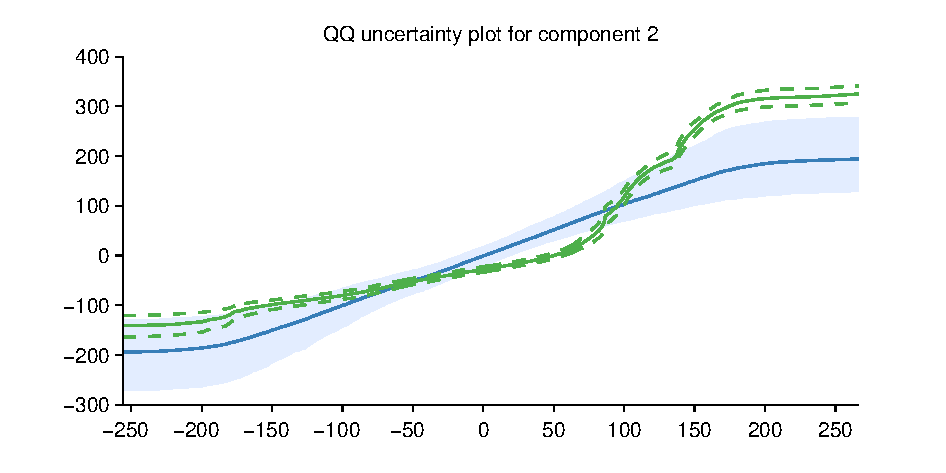
\includegraphics[width=\wmgd,height=\hmgd]{\mdrd/11-unemployment_qq_bands_2}
  \end{tabular}
\end{frame}

\end{document}

\begin{frame}{Title}
  \begin{itemize}
    \item Content
    \vspace{\baselineskip}
    \item Content
    \vspace{\baselineskip}
    \item Content
    \begin{itemize}
       \item Content
       \item Content
     \end{itemize}
  \end{itemize}
\end{frame}
